\documentclass[conference]{IEEEtran}

\ifCLASSOPTIONcompsoc
  \usepackage[nocompress]{cite}
\else
  \usepackage{cite}
\fi

\usepackage[pdftex]{graphicx}
\graphicspath{{../img/}}

\usepackage{color}
\newcommand{\todo}[1]{\textcolor{red}{TODO #1}}

\usepackage[T1]{fontenc}
\usepackage[scaled]{inconsolata}

\definecolor{bluekeywords}{rgb}{0.13,0.13,1}
\definecolor{greencomments}{rgb}{0,0.5,0}
\definecolor{redstrings}{rgb}{0.9,0,0}
\definecolor{mygray}{rgb}{0.5,0.5,0.5}

\usepackage{listings}
\lstset{language=C,
showspaces=false,
showtabs=false,
breaklines=true,
captionpos=b,
numbers=left,                    % where to put the line-numbers
numbersep=-4pt,                   % how far the line-numbers are from the code
numberstyle=\tiny\color{mygray}, % the style that is used for the line-numbers
frame=single,                    % adds a frame around the code
showstringspaces=false,
breakatwhitespace=true,
escapeinside={(*@}{@*)},
commentstyle=\color{greencomments},
keywordstyle=\color{bluekeywords}\bfseries,
stringstyle=\color{redstrings},
basicstyle=\ttfamily\footnotesize,
morekeywords={NUM_SUCCESSORS, NUM_GROUPS},
title=\lstname
}

\begin{document}

\title{A Visualization Framework for Parallelization}

\author{A. Wilhelm,
		V. Savu,
		E. Amadasun,
		T. Schuele,
        and~M. Gerndt}% <-this % stops a space

\author{
	\IEEEauthorblockN{
		Andreas Wilhelm, 
		Victor Savu,
		Efe Amadasun,
		Michael Gerndt \\ 
		\IEEEauthorblockA{
			Technische Unversit\"at M\"unchen\\
			\{wilhelma, savu, amadasun, gerndt\}@in.tum.de
		}
		\and
		Tobias Schuele \\
		\IEEEauthorblockA{
			Siemens Corporate Technology\\%
			tobias.schuele@siemens.com
		}
	}
}

\IEEEtitleabstractindextext{%
\begin{abstract}
Since the advent of multicore processors, developers struggle with the
parallelization of legacy software. Automatic methods are only appropriate to
identify parallelism at instruction level or within simple loops. For most
applications, however, a scalable redesign require profound comprehension
of the underlying software architecture and its dynamic aspects. This leads to
an increasing demand for interactive tools that foster parallelization at
various granularity levels. To cope with this problem, we propose a
visualization framework, and three tailored views for parallelism detection.
The framework is part of \emph{Parceive}, a tool that utilizes dynamic binary
instrumentation to trace C/C++ and C\# programs. The cooperative views allow
identification and analysis of potential parallelism scenarios using seamless
navigation, abstraction, and filtering. In this paper, we motivate our
approach, illustrate the architecture of the visualization framework, and
highlight the key features of the views. A case study demonstrates the
usefulness of Parceive.
\end{abstract}
\begin{IEEEkeywords}
Parallelization, Trace analysis, Software visualization, Program comprehension.
\end{IEEEkeywords}
}

\maketitle

\IEEEdisplaynontitleabstractindextext
\IEEEpeerreviewmaketitle

\section{Introduction}
\label{sec:introduction}
Multicore processors still poses a big challenge to the industry and the
research community. To exploit the increasing processing power of such
processors software parallelism is indispensable. As a result, software vendors
are forced to parallelize their legacy software to make them scalable. Such a
parallelization relies on two essential steps. The first step is to
sufficiently comprehend the given software design and its dynamic behaviour.
The second step is a potential redesign of the software architecture that
enables parallelism. Unfortunately, both steps are tedious and error-prone so
that most of the legacy software still operates sequentially. Besides the
additional complexity of parallel programming, we believe the problem largely
arises due to a lack of appropriate tool support.

In the field of reverse engineering, software analysis tools are invaluable to
understand the structural and behavioral aspects of software systems. These
tools gather necessary data using static (at compilation time) or dynamic
(at runtime) analysis approaches and effectively visualize this data. Dynamic
analysis yields precise information about concrete runtime events. Static
Analysis conservatively reasons over possible behaviors by examining system
artifacts, e.g., source code. It has been cited that hybrid approaches are well
suited to provide good accuracy and soundness of the
analyses~\cite{StaticDynamic}. We implemented Parceive, a tool that combines
static and dynamic analyses to provide effective vies for
parallelization~\cite{Parceive}.

In this paper, we present a visualization framework and two views for Parceive.
Our framework enables efficient analyses on large traces to answer elaborate
user queries. We further support an easy integration of tailored views by
providing a common interface to them. This allows us to address a variety of
viewpoints without writing highly specific analyses. Various optimization and
abstraction techniques in the visualization framework ensure responsiveness and
scalability, e.g., by on-demand loading, caching, trace abstraction, or
communication across views. The two views we present enable users to detect
hotspots, infer parallelization strategies, and validate these strategies
regarding data dependencies.
\section{Parceive}
\label{sec:parceive}
We implemented Parceive, a tracing-based tool for interactive software
analysis~\cite{Parceive}. Its vision is to aid developers with identifying
parallelism opportunities on various granularity levels. Parceive utilizes
static binary analysis and dynamic instrumentation to collect trace data. Being
less conservative than purely static approaches let us focus on
concurrency-related events, e.g., memory accesses, routine invocations, and
object instantiations. By a-posteriori abstraction of such fine-grained
information we infer architectural aspects of user applications. Here is the
difference to most existing tools, the results may be used as a starting point
for an extensive architecture refactoring. However, the user is responsible for
a correct parallelization due to the inherent incompleteness of dynamic
analysis.

\begin{figure}[h!]
	\begin{center}
		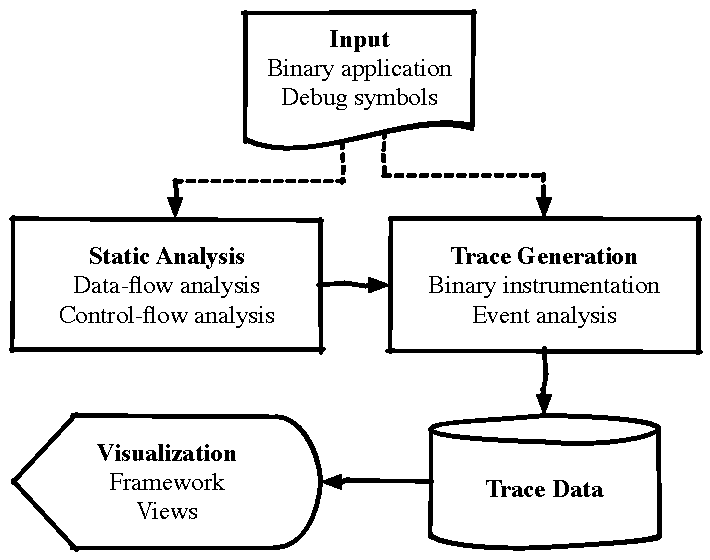
\includegraphics[width=0.40\textwidth]{img/parceive}
		\caption{The high-level components of Parceive.}
		\label{fig:parceive_overview}
	\end{center}
\end{figure}

Figure \ref{fig:parceive_overview} depicts the fundamental components of
Parceive and its relations. Our analyses operate on user applications in
binary form to generate trace data. These analyses can be classified into ones
applied statically and during runtime. The former inspect the data- and
control-flow of single linkage objects. By incorporating given debug
information, static analyses enable our tool to infer global properties, e.g.,
stack variables and their accesses, loop constructs, or class hierarchies.
Additionally, the gathered knowledge is used to tailor the scope of the
subsequent runtime analyses to reduce the execution overhead.

The runtime analyses instrument and inspect predefined events during actual
executions of the user applications, e.g., object instantiations, method
invocations, or thread handling (in case of multi-threaded user applications).
During such events, Parceive collects trace data and efficiently writes it into
a file-based database. The underlying database scheme enables highly specific
and performant queries for visualizations. The visualization component is the
key to comprehend and parallelize user applications. It lets user grasp complex
system behavior by providing views for multiple viewpoints. It consists of a
visualization infrastructure and several views that are based on the
infrastructure. Each view simplifies and highlights specific aspects of the
traced software. We elaborate this in more detail in the next section.
\section{Visualization Component}
In this section, we present certain key aspects of our web-based visualization
component. This component facilitates the integration of arbitrary views to
Parceive by providing a common interface to access abstracted runtime traces.
The biggest challenge when dealing with traces is the potentially overwhelming
amount of data. Often this leads to unmanageable views with unpractical delays.
Our visualization component addresses this problem by building upon a highly
reactive client-server architecture (see Figure \ref{fig:visualization}) that
provides four key services.

\begin{figure}[h!]
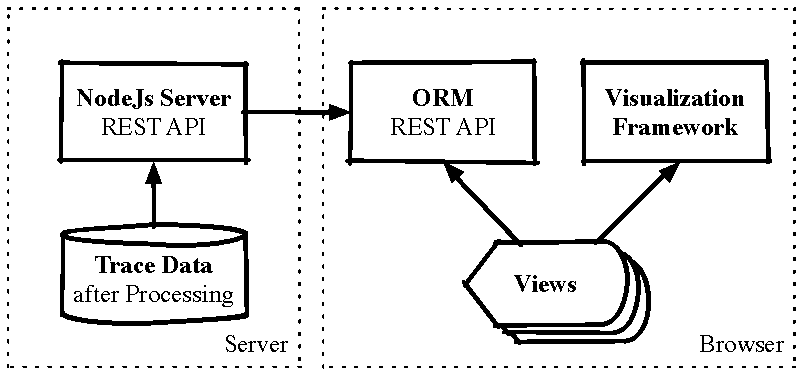
\includegraphics[width=\linewidth]{img/visualization_framework}
\caption{The visualization component of Parceive.}
\label{fig:visualization}
\end{figure}

\paragraph{Trace Optimization}
Parceive uses file-based databases to store trace data. Its
layout is optimized for writing to reduce the runtime overhead. All the
information required by the views can be obtained by using database queries.
However, most of the operations would take a disproportionate amount of time to
complete without applying trace optimization. This step is performed by
post-processing to dramatically reduce lookup times of views.   

Most importantly, the creation of selected indexes dramatically reduces lookup
times by allowing highly optimized search strategies. Since no additional data
will be added to the traces, creating redundancy generates no overhead and does
not increase the complexity. By adding additional fields and creating
intermediary tables, it is possible to avoid joins for most queries executed by
the visualizations. 

Executing \texttt{VACUUM} after all processing is done also improves
performance by reducing the fragmentation of data stored inside tables. The
increased locality of data reduces the execution time of most queries and has a
considerable effect on ones that require a full table scan. \texttt{VACUUM} is
also able to reduce the size of the processed
database.

\paragraph{On-Demand Loading}
The first service that improves responsiveness is on-demand loading of trace
data and its caching for reuse across views. Often, loading entire traces
into the browser is not possible due to memory restrictions. To solve this
problem a NodeJS server was developed that reads data from post-processed 
databases (see Section \ref{dataprocessing}) on demand. The server exposes a
REST \cite{rest} API that manages the retrieval of data. For security reasons
all SQL queries are contained in this server without supporting arbitrary
queries. The implementation makes use of multiple parallel reads to the same
database to reduce the latency and throughput when large amounts of data is
requested by the views. This service enables users to seamlessly navigate and
explore their software across multiple views.

The second service for a better scalability is abstraction of fine-grained
trace information to high-level entities. Examples are function invocations
that are grouped to call-groups, or runtime objects that lead to the
respective classes. 

Such abstractions are enabled by a Object Relational Mapper
(ORM) module to simplify development and improve performance. The ORM makes it
possible to access entities and to easily navigate the relationships
between them. The API is implemented using promises \cite{promises} simplifying
the asynchronous and parallel behavior. 

Such abstractions allow users to better comprehend their
software by using effective top-down approaches. 


The third service comprises a
communication infrastructure for
sharing arbitrary state across multiple views. This service can be used to spot
and restrict the current range of view to crucial points in the trace. Equipped
with all these services, the visualization framework allows scalable views for
software analysis.


\subsubsection*{Performance}

Figure \ref{parceive:procperformance} shows the time and size overhead of
processing databases generated by Parceive. The time required by this operation
is negligible because loading most visualizations without the optimizations
would waste more than the processing itself. The executed queries are also
heavily optimized making \texttt{VACUUM} and the creation of indexes the most
time consuming operations. The size increase is unfortunately unavoidable.

\begin{figure}
	\centering
	\begin{tabular}{l l l l}
		Database & Size & Processed Size & Time taken \\
		emsim\_par & 3905536 & 14560256 & 8.77 s
	\end{tabular}
	\caption{Database processing performance}
	\label{parceive:procperformance}
\end{figure}

\subsection{ORM}



The greatest benefit to using this ORM in visualizations is the possibility of
applying optimizations to the data loading. The most important ones are caching
and pipelining. Caching allows the ORM to avoid loading data that has been
accessed before. Each time an entity is retrieved from the server it is saved
and reused for subsequent requests. This optimization allows visualizations to
focus more on data presentation instead of efficient data retrieval.

Pipelining combines multiple queries to the same endpoint into a single one.
When requesting a large number of entities it can improve performance despite
the limit on the number of parallel requests in browsers. This optimization is
designed to greatly increase throughput at the cost of a response time
increased by 10 milliseconds.

\subsubsection{State management}

The visualization framework implements a centralized and persistent state
storage for visualizations. With the use of this feature it is possible to
retain the state of views across page loads.

Currently the view layout and the marked nodes are stored as part of the state
automatically. In addition to this each visualization can save tailored
information at any time and retrieve it when rendering. Local storage is used
to house all the state information making it persistent.

\subsubsection{Communication}

Visualizations perform different tasks and allow the user to navigate the
callgraph in different ways. Communication makes it possible to follow a chain
of investigation along multiple visualizations. Currently there are three ways
to communicate intent:

\begin{itemize}
	\item[Focus] brings entities to the attention of the user
	\item[Mark] allows the creation of selections that are visible between
visualizations
	\item[Spot] replaces all the entities in a visualization with a new set
	\item[Hover] brings entities to the attention of the user using opacity
\end{itemize}
\section{Views}
In this section, we present three prototypical views that are built upon the
presented visualization infrastructure. The incentive for the users is to
obtain enhanced awareness about available parallelism opportunities. Therefore,
the interaction of the views provide a scalable top-down approach to identify
hotspots, develop parallelization strategies, and validate these strategies for
data dependencies. In the following Sections, we list the suggested views of
this paper.

\subsection{Performance View}
\label{sec:performance_view}
The performance view is a interactive representation of a program's profiling
and trace data. Its primary purpose is to assist users in identifying scenarios
that could potentially improve performance, by employing parallel programming
as an optimization solution. Tracing and profiling provide valuable material
for detailed analysis on how a program behaves at runtime. Presenting a
wholistic view of this data in an easy to digest visualization, can help users
quickly comprehend the program behavior, spot potential performance
bottlenecks, and help guide optimization efforts.

Two visualization modes are provided in the performance view: tracing and
profiling. The tracing mode represents an icicle plot extended with loop
information, i.e., a hierarchical view of calls made during program execution.
The calls are arranged from left to right chronologically, and the visibility
of the loop information for each loop execution can be toggled on or off. The
trace visualization is useful for detailed examination of a program, especially
where the traced invocation order is important. The profiling mode presents the
user a hierarchical view of the functions called during a program's execution.
The length of each function in the view is dictated by the sum of the duration
of calls made to it. The profiling visualization is often sufficient to quickly
pinpoint hot spots.

As user programs grow in size and complexity, the performance data also grows,
and becomes harder to digest all at once. Which is why the performance view
provides zooming on call level and runtime duration filtering, to help the
user adjust the view to different data granularity levels. Runtime duration
filtering sets the minimum runtime duration required for a call to be loaded.
The minimum runtime duration value is gotten by calculating a specified
percentage of the runtime duration of the current top-level call in the view.
This feature allows the render only calls large enough to be easily visible.
With the call zooming feature, users can focus the view on a specific call,
which then makes it the top-level call, re-computes a new minimum runtime
duration, and loads any child calls of the focused call that wasn't visible due
to the previous runtime duration constraint.

\begin{figure*}[ht!]
	\begin{center}
		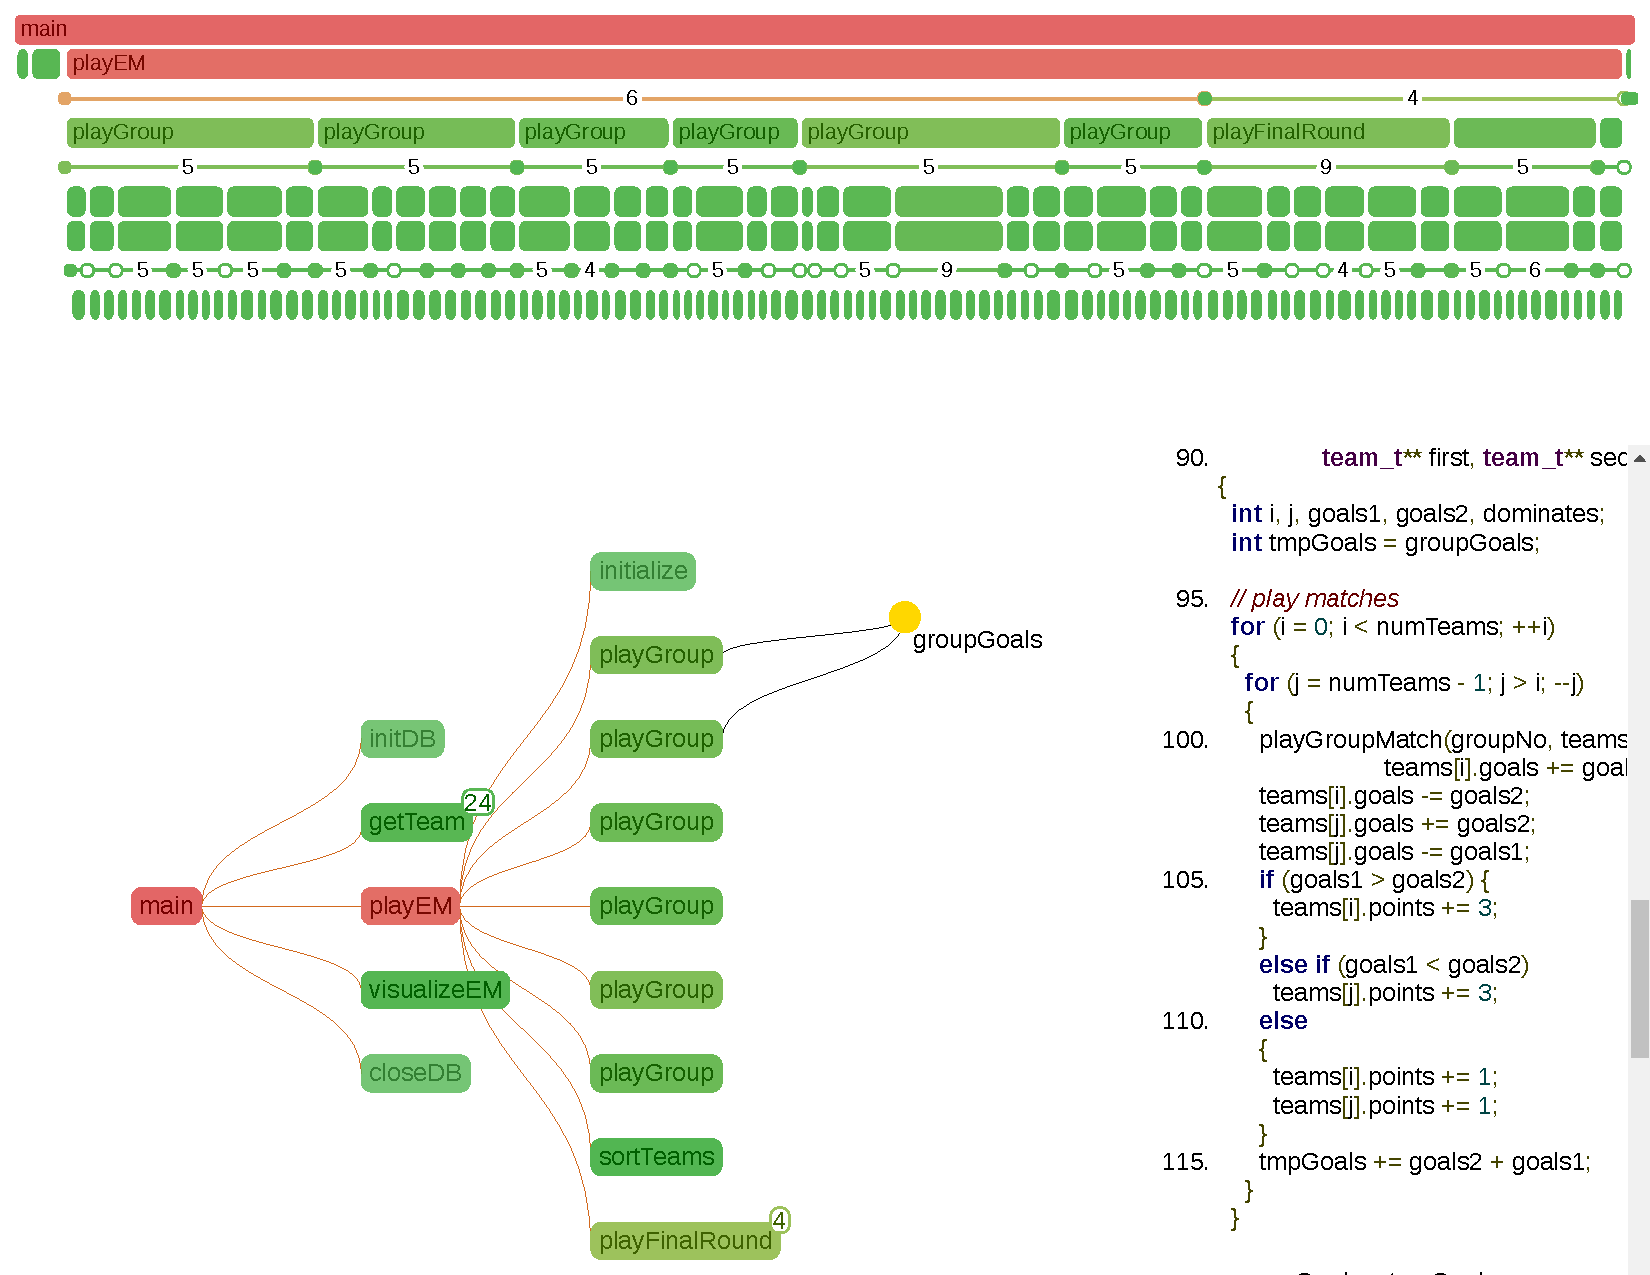
\includegraphics[clip, trim=0.1cm 16.0cm 0.1cm 0.1cm,
width=\linewidth]{img/performance_view.pdf}
		\caption{The performance view of Parceive showing an EMSim trace.}
		\label{fig:emsim}
	\end{center}
\end{figure*}

\subsection{Calling Context Tree (CCT) View}
The CCT view is a visualization that aids the comprehension of dynamic behavior
of an application. The view can display a call tree consisting of call nodes
that is extended with loop nodes and referenced memory nodes (see Figure
\ref{fig:cct_view}). Nodes for calls (or group of calls), loop executions and
loop iterations are positioned using a tidy tree layout~\cite{TidierTree}.
Children of nodes are vertically sorted by their start time to facilitate
comprehension of traced executions. Memory nodes accessed by arbitrary tree
nodes are difficult to integrate as part of a tree layout. Hence, we positioned
these nodes using an unconstrained layout that is based on a force simulation
around the rest of the tree.

The first node present when the view is created is the call to the
\texttt{main} function. Users can arbitrarily expand and collapse call nodes.
When a function was called multiple times during the same function execution,
the respective call nodes are grouped to so-called \textit{call groups}. Call
groups reduce the number of nodes to be displayed but can also be decomposed
into their single call nodes. Navigating loop executions and loop iterations is
similar to calls and allows the user to see information at any desired
granularity. 

For parallelization, the most important feature of the CCT view is data
dependency analysis. Users are often interested in the existence and the
locations of such dependencies between arbitrary regions of their software.
Therefore, a optimized query of the visualization infrastructure is utilized
to detect shared memory accesses across deep call hierarchies. Found
dependencies can then be inspected in a separate source code view. The
described feature allows manageable visualizations by dramatically reducing the
amount of shown nodes. There are some additional features that aim for better
scalability and to help developers parallelizing code:

\begin{itemize}
	\item Profiling information (relative execution time) is present by node
colors.
	\item Exposing and collapsing entity nodes can be performed in both
directions, i.e., to show and hide parent or children nodes.
	\item Seamless zooming or panning, and focusing on single entity nodes for
a clear visualization.
	\item Spotting of arbitrary call nodes that automatically expands the call
tree up to these nodes and start with their common ancestor.
\end{itemize}

\begin{figure}[h!]
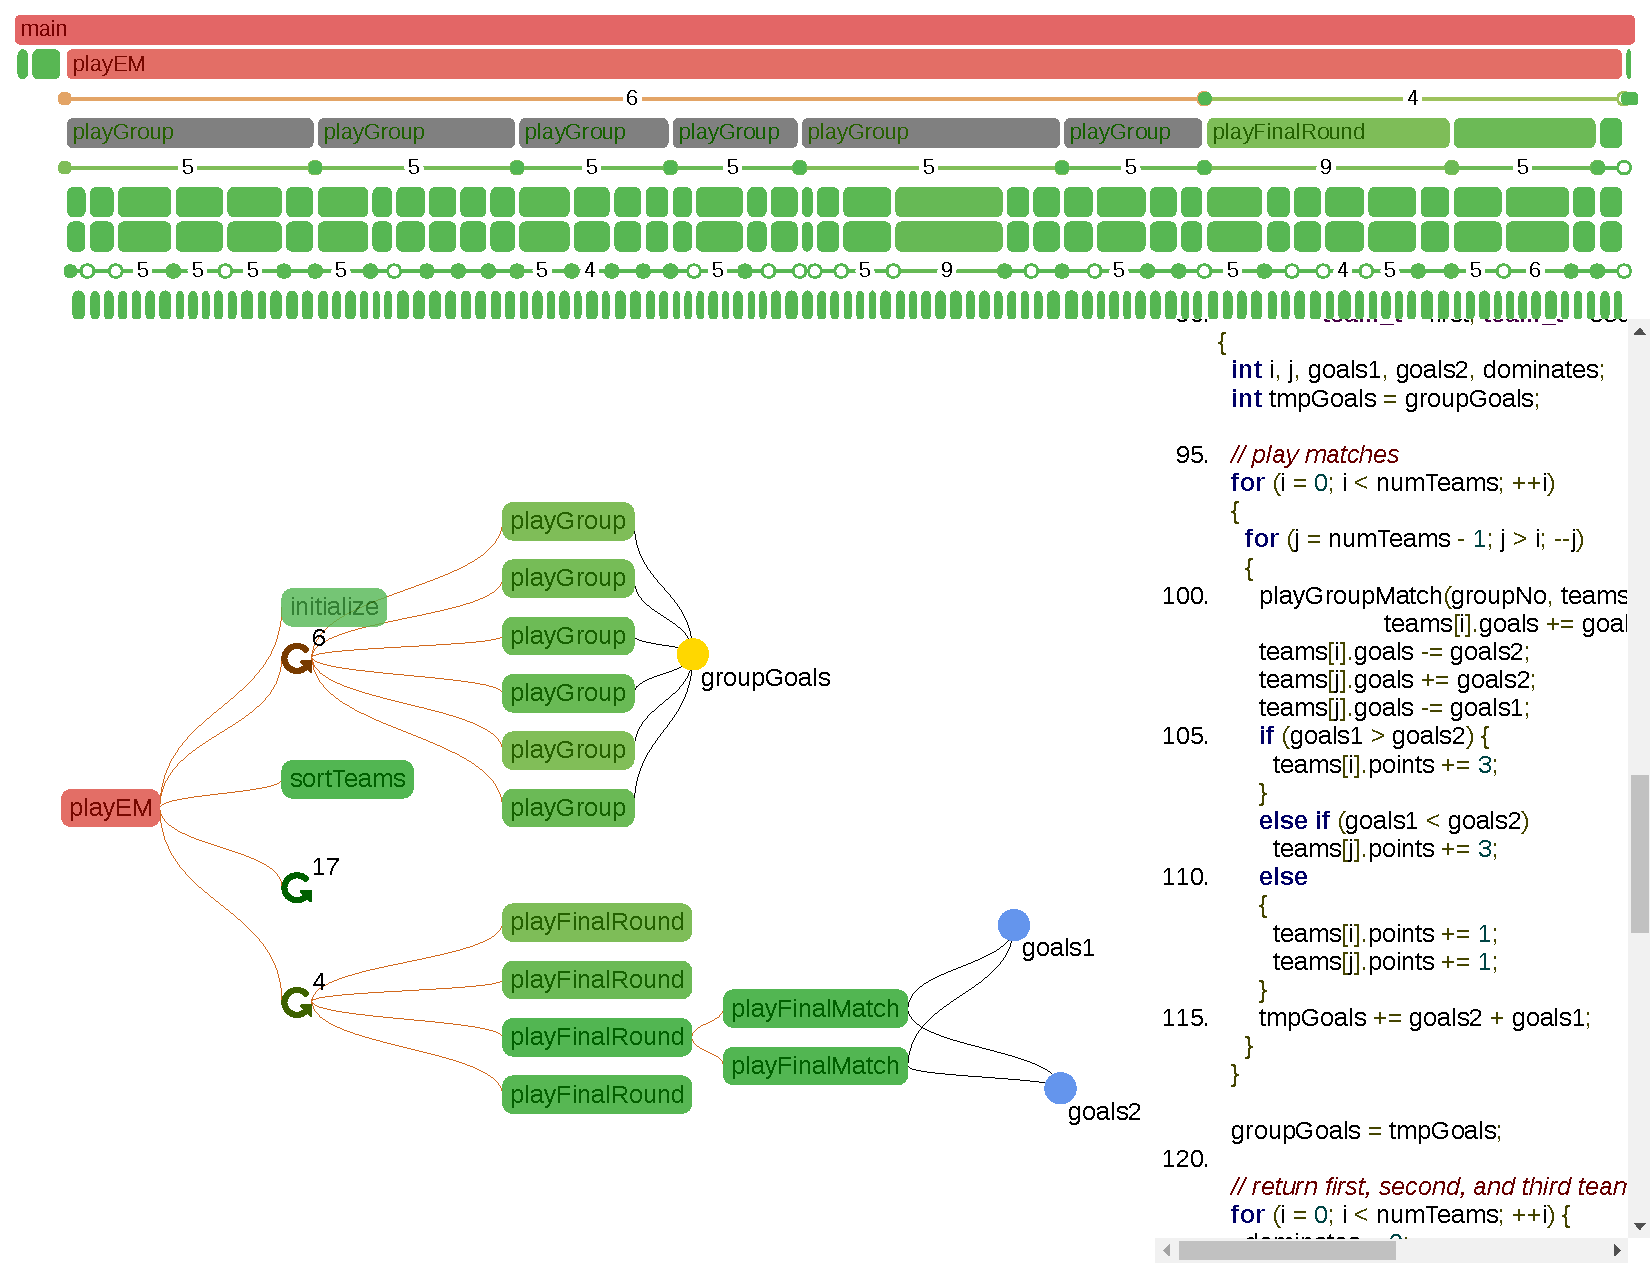
\includegraphics[clip, trim=0.9cm 2.5cm 8.5cm 8.5cm,
width=\linewidth]{img/cct_view}
\caption{The calling context tree view of Parceive.}
\label{fig:cct_view}	
\end{figure}


\subsection{Source View}
The source view shows the highlighted source code in a file that was used to
build the instrumented application.The usefulness of this view becomes apparent
when it is communicating with the others presented in this paper. The simplest
interaction is focusing and it allows the source view to pinpoint the
definition of functions, loops, and memory accesses that makes it easy to
follow the execution of a program trough the source code. Hovering is able to
provide additional information about entities. For calls it can indicate where
the call originated and for memory references where they were allocated and
referenced.
\section{Case Study: EMSim}
\label{sec:case_study}
In this section, we demonstrate Parceive by applying it to EMSim, a simulator
for the European soccer championship. EMSim was part of the student assignments
for a master course on parallel programming. The application simulates all
matches by relying on historical statistics of results, teams, and players. The
task was to parallelize the sequential C code by considering the following
steps: (1) the comprehension of EMSim and its behavior, (2) the location of
hotspots, (3) the identification of dependencies, and (4) the parallelization
with appropriate libraries. The students were able to upload their source code
to a submission server for checking correctness and speedup. As it turned out,
the biggest challenges were to estimate the load balance and to identify data
dependencies. In the following, we show that Parceive helps with both issues.

\begin{lstlisting}[caption=A major region for loop-parallelism in the
EMSim code, label=listing:playEM]
  // play groups
  for (int g = 0; g < NUM_GROUPS; ++g) {
    playGroup(
      teams + g,
      successors + (g * 2),
      successors + (NUM_SUCCESSORS - (g * 2) - 1),
      bestThirds + g
    );
  }
\end{lstlisting}

Listing \ref{listing:playEM} is an excerpt of the EMSim code that contains a
major opportunity for parallelism. The shown loop is contained in the
\texttt{playEM()} function, which gets arrays of teams as input. Every
iteration calls \texttt{playGroup()} for each group of the preliminary round,
which simulates the matches between the given teams and returns the first,
second, and third winning team. This loop accounts for \textasciitilde60\% of
the overall runtime. Even though the loop is easily identified as an
opportunity for parallelization, the crux is to analyze dependencies between
the calls. The first challenge is to understand the pointer arithmetic in lines
5 and 6, which scatters qualified teams to the successor array. The second
challenge is to inspect the (arbitrarily deep) call paths for accesses to
common memory locations.

We applied Parceive to EMSim by tracing an execution of the optimized user
binaries. The instrumentation framework and the runtime analyses caused an
execution slowdown factor of \textasciitilde 4.4 (20s instead of 4,5s). The
produced trace data had a size of 4.3Mb, where data about memory accesses and
function invocations account for 84\% of the size. After producing the trace
database, we imported it to our visualization infrastructure.

The trace view that depicts the execution of EMSim is shown in Figure
\ref{fig:emsim}. The call of \texttt{main()} spends most of the time in the
invocation of \texttt{playEM()}. Within this function call, the execution time
is mainly spent within two loops. The first loop (the one from
Listing~\ref{listing:playEM}) simulates the preliminary round. The second loop
simulates the final rounds, from the round of 16 to the final match.

Recall the two main purposes of the trace view, namely identifying hotspots
and estimating load balance. In the case of EMSim, the view indicates the
invocations of \texttt{playGroup()} and \texttt{playFinalRound()} as
significant hotspots. Without considering dependencies, a naive strategy is to
invoke the single calls by individual threads. Besides limited scalability
(there are only 6 calls of \texttt{playGroup()}), this solution results in a
non-optimal load balance since the calls vary in their execution time. However,
the trace view exposes another opportunity for parallelism. Both the group
matches and the final matches lead to distinct calls of
\texttt{playMatchGeneral()} (not shown due to space constraints). Hence, a
second strategy is to use a master-worker pattern for scheduling these calls
with a thread-pool. The next step for the user is to validate the found
parallelization strategies.

The CCT view supports users with the validation of prospective refactorings. 
Figure \ref{fig:cct_view} shows the resulting view for EMSim. Notice that
only relevant call nodes for the investigated parallelization strategies are
shown by spotting them on the trace view. Beginning with the first strategy, we
are interested in possible data dependencies between the invocations of
\texttt{playGroup()} and \texttt{playFinalMatch()}, respectively. The
corresponding analysis (\textit{show deep dependencies}) queries accesses 
to common memory locations among full call paths. It turns out that each
invocation of \texttt{playGroup()} accesses the global variable
\texttt{groupGoals} and each invocation of \texttt{playFinalMatch()} accesses
the stack variables \texttt{goals1} and \texttt{goals2}. Furthermore, the CCT
view enables us to localize these memory accesses in the source code so that
the dependencies can be resolved.

Even though the data dependencies for the first parallelization strategy
can be easily avoided, we focus on the second strategy that puts the calls to
\texttt{playMatchGeneral()} in distinct tasks. Performing the same dependency
analysis as before returns no shared memory accesses between these calls (not
shown due to space constraints). Hence, the user gains the necessary
information to parallelize EMSim by integrating the master-worker pattern. A
student solution achieved a speedup of 6.5 on our 8-core system. Considering
some sequential pre- and post-processing steps, and the control dependencies
between certain matches (e.g., the semi-final has to be played before the
final), the gained speedup confirms Amdahl's law~\cite{amdahl}. These results
conclude that our views are very helpful for parallelization.

\section{Related Work}
\label{sec:related_work}
Trace visualization has a long history in analyzing software
parallelism~\cite{TraceVisualization}. Current visualizations are able to
handle up to $10^7$ events or terabytes of trace data~\cite{State}. However,
most of the cited methods achieve these numbers only for statistical plots or
by averaging pixels. Others gain scalable views at the expense of limited
usability, e.g., by requiring users to extensively pan across detailed trace
data. Our tool tries to create the sweet spot between full abstraction and
largely unprocessed details through a more interactive approach.

Vampir and HPCToolkit are tools from the performance community that provide
visualization environments to represent performance data~\cite{Vampir,
HPCToolkit}. This enables a detailed understanding of dynamic processes on
massively parallel systems. Vampir handles terabytes of data via parallel1
preprocessing and data reduction techniques during collection. HPCToolkit
maintains interactivity of its views by sampling the data rather than on-demand
processing during panning and zooming. Both tools focus on parallel software to
highlight performance and communication issues. In contrast, the intention of
Parceive is to aid with parallelization of legacy applications.

Moose certainly belongs to the most prominent reverse engineering
frameworks~\cite{Moose}. It provides a set of services including a common
meta-model, metric evaluations, a model repository, and generic GUI support for
querying, browsing and grouping. Metric results can arbitrarily visualized by a
set of views, e.g., polymetric views, evolution matrices, or butterfly views.
Though the functionality of Moose by far exceeds the one of our tool, we often
rely on highly optimized search strategies (e.g., deep dependency analysis) and
specialized views for parallelization.
\section{Future Work}
\label{sec:future_work}
Parceive was developed using a data-centric approach, where the initial project
phase focused on fine-grained trace data and its visualization. In the second
project phase, we will apply abstraction on this data to gain architectural
insights for software comprehension and parallelization. Additional knowledge
from software architects and developers will be incorporated to specify
software components. This knowledge can then be used for extended views that
depict the structure of systems and their behaviour on architecture level.

Currently, we are working on multiple features that improve the usability of
Parceive, or even extend possible uses. One such feature are views that depict
parallel behavior of multi-threaded applications. Possible use-cases are
scalability analysis or validation, e.g., to identify possible race conditions.

We reviewed the visualization component on a few open and closed source
applications, some of them are at industrial scale. The tests focused on the
scalability of the framework and the effectiveness of the views. However, more
tests are necessary to measure performance and responsiveness, and to elicit
possible scaling problems. We plan to focus on an extensive set of sequential
user applications with decent parallelism potential.
\section{Conclusion}
\label{sec:conclusion}
Visualization of software behavior is a crucial instrument to comprehend
software systems. Unfortunately, this task often involves an overwhelming
amount of trace data that easily overstrains current UIs. Therefore, we built a
highly scalable and responsive visualization infrastructure for our tracing
tool Parceive. The core is a client-server architecture providing asynchronous
event driven data retrieval and optimized analysis queries. These techniques
empower users to explore and navigate their traced applications by multiple
viewpoints. This paper additionally presented three views that aids with
identification and validation of potential parallelism scenarios. Currently, we
are in an early stage of research. Future work will mainly cover higher-level
aspects to comprehend software systems in a top-down approach.
%
\section*{Acknowledgements}
We thank Nathaniel Knapp for comments and suggestions. Additionally, we
gratefully acknowledge the support of Siemens. This work has been supported by
the German Federal Ministry of Education and Research (Software Campus, grant
no. 01IS12057).
%

\bibliographystyle{abbrv}
\bibliography{biblio}

\end{document}


